\documentclass[titlepage,a4paper]{article}

\usepackage{a4wide}
\usepackage[colorlinks=true,linkcolor=black,urlcolor=blue,bookmarksopen=true]{hyperref}
\usepackage{bookmark}
\usepackage{fancyhdr}
\usepackage[spanish]{babel}
\usepackage[utf8]{inputenc}
\usepackage[T1]{fontenc}
\usepackage{graphicx}
\usepackage{float}
\usepackage{listings}
\usepackage{xcolor}

																	% VARIABLES 

\newcommand{\FirstName}{Carlos E.}
\newcommand{\LastName}{Castillo}
\newcommand{\StudentID}{108535}
\newcommand{\StudentEmail}{ccastillo@fi.uba.ar}
% \newcommand{\ProjectName}{Trabajo Práctico n — NombreTP}
\newcommand{\ProjectName}{TDA 3 — Hash}

\pagestyle{fancy}
\fancyhf{}
\fancyhead[L]{TP - \FirstName \LastName}
\fancyhead[R]{Algoritmos y Programación II - FIUBA}
\renewcommand{\headrulewidth}{0.4pt}
\fancyfoot[C]{\thepage}
\renewcommand{\footrulewidth}{0.4pt}

\definecolor{codegreen}{rgb}{0,0.6,0}
\definecolor{codegray}{rgb}{0.5,0.5,0.5}
\definecolor{codepurple}{rgb}{0.58,0,0.82}
\definecolor{backcolour}{rgb}{0.95,0.95,0.92}

\lstdefinestyle{mystyle}{
    backgroundcolor=\color{backcolour},   
    commentstyle=\color{codegreen},
    keywordstyle=\color{magenta},
    numberstyle=\tiny\color{codegray},
    stringstyle=\color{codepurple},
    basicstyle=\ttfamily\footnotesize,
    breaklines=true,                 
    captionpos=b,                    
    keepspaces=true,                 
    numbers=left,                    
    numbersep=5pt,                  
    tabsize=4
}

\lstset{style=mystyle}

\begin{document}
\begin{titlepage}
	\hfill
\includegraphics[width=6cm]{logofiuba.jpg}
    \centering
    \vfill
    \Huge \textbf{\ProjectName}
    \vskip2cm
    \Large [7541/9515] Algoritmos y Programación II\\
    Segundo cuatrimestre de 2021 
    \vfill
    \begin{tabular}{ | l | l | }
      \hline
      Alumno: & \LastName, \FirstName \\ \hline
      Número de padrón: & \StudentID \\ \hline
      Email: & \StudentEmail \\ \hline
  	\end{tabular}
    \vfill
    \vfill
\end{titlepage}

\tableofcontents
\newpage

																 % INTRODUCCION

\section{Introducción}\label{sec:intro}

Muchos lenguajes de programación permiten al usuario extender los tipos de datos
nativos del lenguaje con para facilitar la implementación de características y
funcionalidades más complejas. De esta forma, el programador tiene la capacidad
de combinar diferentes primitivas del lenguaje y así generar nuevos tipos
compuestos para crear interfaces abstractas que faciliten el manejo y
organización de la información mediante diferentes estructuras de datos.

El objetivo de este trabajo práctico es implementar una de las estructuras de
datos más utilizadas, la tabla de hash. 

                                    % TEORIA

\section{Teoría}\label{sec:teoria}

\subsection{Tabla de Hash}

El concepto de tabla de hash se deriva de la estructura de datos conocida como
diccionario, una colección de pares clave-valor, en la que cada elemento está
asociado con una clave única con la que es identificado una vez es almacenado en
el diccionario. De esta forma para acceder a los elementos contenidos en el
diccionario se utiliza la misma clave con la que se insertó. Esta estructura de
datos y sus derivados son utilizados principalmente por su capacidad de acceder
rápidamente a la información y evitar la duplicidad de entradas.

\begin{figure}[H]
\centering
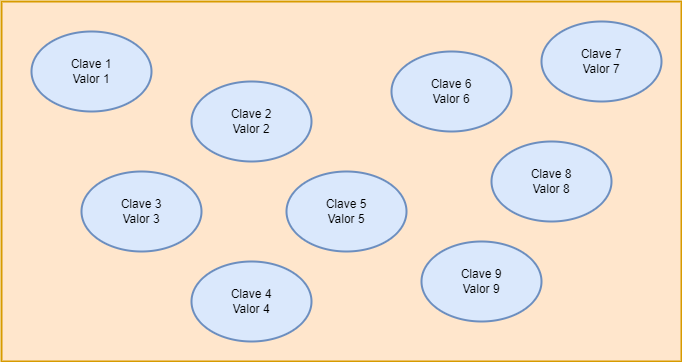
\includegraphics[width=0.8\textwidth]{img/1_diccionario.png}
\caption{\label{fig:seq01}Estructura de Datos Diccionario.}
\end{figure}

En particular una tabla de hash implementa un arreglo asociativo en el que la
ubicación de cada elemento agregado es calculada a traves de una función de
hash, la cual genera un índice dentro del arreglo a partir de la clave
indicada.  Así para insertar, acceder o quitar un elemento almacenado en la
tabla, se toma la clave provista, se encuentra su índice a través de la función
de hash y finalmente se accede a esa posición dentro de la tabla. 

Sin embargo, a medida se van agregando elementos a la tabla, se va aumentando
la probabilidad de que para dos claves distintas se genere un mismo indice de
hash. Cuando esto sucede se dice que hay una ''colisión''. Existen muchas
alternativas para resolver estas colisiones, la mayoría de las cuales implican
cambiar ligeramente la estructura de la tabla o requieren de algún tipo de
reorganización de la información ya almacenada. Las variantes de tablas de hash
más comunes para lidiar con colisiones son la tabla de ''hash abierto'' y tabla
de ''hash cerrado''. 

													 \subsection{Hash Abierto}

Una tabla de hash abierto consiste en una tabla de hash capaz de hacer
encadenamiento o ''chaining'' a los elementos con un mismo indice de hash. Para
esto se suele implementar una estructura de datos secundaria en la que se
almacenarán los elementos que colisionen, generalmente listas enlazadas. De
esta forma la tabla de hash en sí solamente contiene referencias a las
diferentes listas en las que se guardan los elementos. Cada indice de hash
apunta más bien a cada una de estas listas y en caso de colisión, dos pares
clave-valor con el mismo indice de hash van a ser almacenados en la misma
posición en la tabla de hash y encadenados al final de la lista en esa
posición.

\begin{figure}[H]
\centering
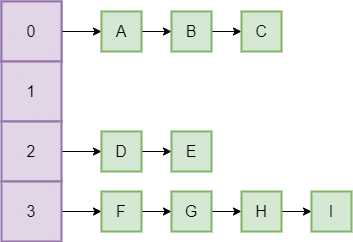
\includegraphics[width=0.5\textwidth]{img/2_hash_abierto.png}
\caption{\label{fig:seq02}Hash Abierto con Listas Enlazadas.}
\end{figure}

Sin embargo uno de los puntos negativos de utilizar este tipo de hash es que
si se van insertando varios elementos con el mismo indice de hash, las listas
enlazadas van a ir aumentando su longitud, haciendo que el tiempo de acceso a
los elementos se tienda a ser $O(n)$ en vez de conservarse como $O(1)$ como es
característico de las estructuras de datos diccionarios. Para evitar esto se
suele hacer una operación conocida como ''rehash'' cuando la cantidad de
elementos en una tabla de hash sobrepasa cierto umbral. Esta operación consiste
en incrementar el número de listas en la tabla y reinsertar nuevamente los
elementos almacenados, ya que al si el indice producido por la función de hash
depende de la cantidad de listas disponibles, al incrementar dicha cantidad,
los indices de elementos previamente almacenados deberán ser reasignados en
base a la nueva cantidad de listas disponibles.

													% DETALLES DE IMPLEMENTACION

				 \section{Detalles de implementación}\label{sec:implementacion}

La implementación de esta estructura de datos fue escrita en el lenguaje de
programación C, siguiendo la especificación del lenguaje detallada en el
estándar C99. Los archivos principales se encuentran dentro del directorio
\textbf{src} ubicada en la raíz del repositorio. 

Además se incluye un archivo \textbf{pruebas.c} en el que se encuentran
diferentes pruebas automatizadas para detectar errores en la ejecución del
programa o en la asignación, manejo y liberación de memoria dinámica. Para esto
se utiliza \textbf{gcc} como compilador y \textbf{valgrind} como herramienta de
análisis de memoria.

La estructura de tabla de hash propuesta para esta implementación es la
siguiente:

\begin{lstlisting}[language=C]
struct hash {
	casilla_t** casillas;
	size_t cantidad_casillas;
	size_t cantidad_elementos;
	hash_destruir_dato_t destruir_elemento;
};
\end{lstlisting}

El campo \lstinline{casillas} de cada hash es un vector de listas simplemente enlazadas y puramente recursiva, implementadas de la siguiente forma:

\begin{lstlisting}[language=C]
typedef struct casilla {
	char* clave;
	void* elemento;
	struct casilla* siguiente;
} casilla_t;
\end{lstlisting}

Al estar utilizando esta segunda estructura de datos, la mayoría de las operaciones de la tabla de hash son fundamentalmente auxiliares que trabajan
con operaciones de lista enlazada, por lo que el funcionamiento de las mismas es muy similar al de las operaciones regulares para una lista enlazada.

                         \subsection{Insertar Elemento}

Para insertar elementos en el hash se provee la función
\lstinline{hash_insertar} que recibe la clave y el elemento a insertar. Lo
primero que se hace en este caso es determinar la posición en la que se va a
insertar el elemento dentro de las posiciones disponibles en el vector de
casillas de la tabla de hash. Para esto se utiliza como auxiliar la función
\lstinline{calcular_indice_hash}, que toma la clave dada y retorna la sumatoria
de los valores ASCII de cada uno de los caracteres de esta clave. A este
resultado luego se le aplica la operación módulo respecto del tamaño actual del
vector de casilleros del hash, para así limitar el índice de hash a un rango
válido para este vector.

\begin{figure}[H]
\centering
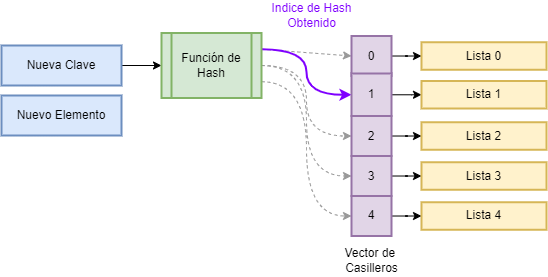
\includegraphics[width=0.8\textwidth]{img/3_hash_insercion.png}
\caption{\label{fig:seq03}Inserción de clave con función de hash.}
\end{figure}

Una vez se determina el indice correspondiente, se llama a la operación insertar
de la lista enlazada ubicada en ese índice. Para esto se utiliza la función
\lstinline{casilla_insertar} que recorre la lista deseada de manera recursiva
hasta encontrar la clave dada o hasta llegar al final de la lista. Si encuentra
la clave dada antes de llegar al final de la lista, significa que esa clave ya
tenía asignado un elemento previamente, así que destruye ese elemento para
actualizar la clave en cuestión con el nuevo elemento que se desea guardar.  En
el caso de que se llegue al final de la lista sin haber encontrado la clave, se
crea un nuevo nodo/casilla en la que se guarda una copia de la clave y se
almacena el elemento.

                             \subsubsection{Rehash}

Para evitar la degeneración excesiva causada por la continua inserción de
múltiples claves con el mismo valor de hash, se implementa también una operación
interna de rehash. Esta se encarga de reorganizar el hash original,
incrementando la cantidad de listas disponibles y volviendo a insertar los
elementos almacenados. Esta función primero crea una copia del estado original
del hash. Luego agranda el tamaño del vector de casillas y le asigna una nueva
ubicación en memoria, lo suficientemente grande para el nuevo tamaño del hash.
Sin embargo al reasignar la memoria, el vector en cuestión pierde toda la
información que estaba almacenada, por lo que se debe recurrir a la copia hecha
previamente para ir insertando los elementos uno a uno. Esto se hace con la
ayuda de la función \lstinline{casilla_copiar_casillas}, la cual va recorriendo
cada una de las listas recursivamente y llamando a la función
\lstinline{casilla_insertar} para cada elemento.

La operación de rehash es computacionalmente costosa, así que solo se manda aplica cuando la cantidad de elementos almacenados en el hash supera determinado umbral en relación con la capacidad total del mismo. En este caso el umbral es:

$$
\frac{\textnormal{cantidad\_elementos}}{\textnormal{cantidad\_casillas}} \ge 0.75
$$

Y el factor de incremento al aumentar la cantidad de espacios disponibles en el hash anterior es igual a $2$, es decir, cada vez que se hace rehash, la cantidad de listas en el hash se duplica.

                          \subsection{Quitar Elemento}

La operación de quitar un elemento se asemeja a la de insertar. En esta
operación nuevamente lo primero que se hace es calcular el índice de hash que
corresponde con la clave dada. Luego se ubica la lista que se encuentra en ese
índice y se utiliza la función \lstinline{casilla_quitar} para eliminar la clave
deseada de la lista.  La operación de quitar un elemento se asemeja a la de
insertar. En esta operación nuevamente lo primero que se hace es calcular el
índice de hash que corresponde con la clave dada. Luego se ubica la lista que se
encuentra en ese índice y se utiliza la función \lstinline{casilla_quitar} para
eliminar la clave deseada de la lista.

                         \subsection{Iterador Interno}

La función \lstinline{hash_con_cada_clave} permite recorrer los elementos de un hash y aplicarles un función a cada elemento. Para esto se utiliza una función auxiliar \lstinline{casilla_con_cada_clave} que simplemente recorre cada lista enlazada de manera recursiva. Esta función se manda a llamar para cada lista almacenada en el vector de casillas del hash. En caso de que la función aplicada sobre un elemento retorne \lstinline{true} se detiene el recorrido del hash.

\begin{figure}[H]
\centering
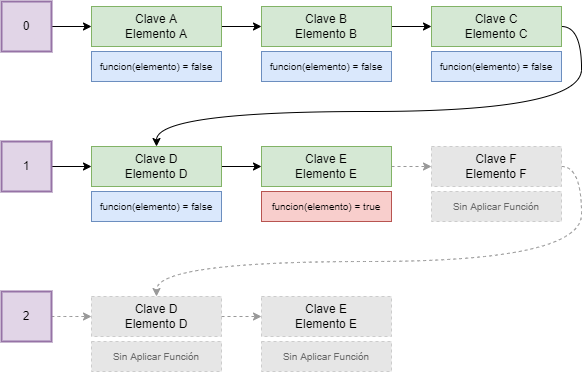
\includegraphics[width=0.8\textwidth]{img/4_recorrido.png}
\caption{\label{fig:seq04}Recorrido hasta que función retorne \lstinline{true}.}
\end{figure}

                         \subsection{Otra Operaciones}

Además de las operaciones de insertar y quitar se provee la función
\lstinline{hash_contiene} que solamente verifica si existe una clave dada en el
hash, los getters \lstinline{hash_obtener} y \lstinline{hash_cantidad}, la
primera de estas funciones se encarga de buscar un elemento por su clave y
retornarlo si lo encuentra, la segunda devuelve la cantidad total de elementos
almacenados actualmente en el hash. Tanto \lstinline{hash_contiene} como
\lstinline{hash_obtener} utilizan funciones auxiliares recursivas que recorren
las listas enlazadas para encontrar la clave dada.

También se proveen las funciones encargadas de la creación y destrucción de una tabla de hash. La función \lstinline{hash_crear} toma una cantidad inicial de casillas mayor a $3$ o directamente el valor $3$ si el valor dado es menor. En base a la cantidad inicial de casillas también se asigna la memoria correspondiente, inicializando todas las listas enlazadas (todas inician como NULL). Finalmente se guarda una función \lstinline{destruir_elemento} que va a ser utilizada al momento de la liberación de un elemento, y se inicia la cantidad actual de elementos insertados en $0$. Por otra parte, la función \lstinline{hash_destruir} utiliza la función auxiliar \lstinline{casilla_destruir} para destruir cada lista enlazada recursivamente, destruyendo cada uno de los elementos con la función \lstinline{destruir_elemento} que se asigna en la creación del hash.

\end{document}

